
%% Template by Michal Forisek


\documentclass[12pt,a4paper]{report}
%\usepackage{slovak}
\usepackage[utf8]{inputenc}
\usepackage[IL2]{fontenc}
%\usepackage{a4wide}
\usepackage{tabularx}
\usepackage{amsfonts}
\usepackage{amssymb}
\usepackage{amsmath}
\usepackage{amsthm}
\usepackage{mathtools}
%\usepackage{breqn} % messes up biblatex and \log_2
%\usepackage{epsfig}
\usepackage{color}
\usepackage{mathrsfs}
\usepackage{verbatim}
\usepackage{fancyvrb}
\usepackage{float}
\usepackage{longtable}
\usepackage{listings}
\usepackage{graphicx}
\usepackage{changepage}
\usepackage{caption}
\usepackage{subcaption}
\usepackage{multirow}
\usepackage{paralist}
\usepackage{pdfpages}
\usepackage{tikz}
\usepackage{pgfplots}
\usepackage{gnuplot-lua-tikz}
\usetikzlibrary{arrows}
\usetikzlibrary{positioning}
\usetikzlibrary{shapes}
\usetikzlibrary{calc}
\usetikzlibrary{decorations.pathreplacing}
\usetikzlibrary{backgrounds}
\usetikzlibrary{fit}
\usepackage[style=alphabetic,maxbibnames=47,backend=biber]{biblatex}
\input{utility/makra.tex}

\def\author{Michal Petrucha}
\def\supervisor{RNDr. Michal Forišek, PhD.}
\def\titlea{Selected Topics}
\def\titleb{from Advice Complexity}
\def\title{\titlea{} \titleb}
\def\thesistype{Diploma thesis}
\def\year{2014}
\def\location{Bratislava}
\def\department{Department of Computer Science}
\def\studyprogram{Informatics}
\def\fieldnumber{2508}
\def\university{Comenius University in Bratislava}
\def\faculty{Faculty of Mathematics, Physics and Informatics}

\usepackage[hidelinks]{hyperref}

\addbibresource{literature.bib}

\newlength{\firstpagewidthinc}
% The length by which we want the first two pages wider:
\setlength{\firstpagewidthinc}{2cm}
\graphicspath{{img/}}
\linespread{1.3}

\lstset{numberstyle=none, basicstyle=\ttfamily,
showstringspaces=false, escapechar=\%, language=C++}

% TODO: Move the setup of packages into a separate file.

% Set up hyperref...
\hypersetup{
    pdfauthor = {\author},
    pdftitle = {\titlea{} \titleb},
    pdfkeywords = {online problem} {advice complexity} {approximation}
}

% TikZ setup for DPA and other graph figures.
\tikzstyle{vertex} = [circle, thick, draw, inner sep = 2]
\tikzstyle{full vertex} = [vertex, fill = black]
\tikzstyle{empty vertex} = [vertex, fill = white]
\tikzstyle{path vertex} = [full vertex]
\tikzstyle{query vertex} = [empty vertex]
\tikzstyle{edge} = [thick]
\tikzstyle{graph picture} = [scale = .7]
\tikzstyle{background highlight} = [rounded corners = 1ex,
                                    fill = black!30,
                                    transform shape,
                                    inner sep = .5em,
                                   ]

\begin{document}

\newlength{\firstpagewidth}
\setlength{\firstpagewidth}{\textwidth}
\addtolength{\firstpagewidth}{\firstpagewidthinc}

\pagenumbering{roman}

%%%%%%%%%%%%%%%%%% Obal %%%%%%%%%%%%%%%%%%
\thispagestyle{empty}
% Tu je kopa zakomentovanych riadkov, lebo Pastorovej sa z nejakeho dovodu
% nepaci v niektorych pracach, ze maju na obale logo, zatial co pri inych
% jej to vobec nevadi, tak nech je spokojna.
\begin{adjustwidth}{-0.5\firstpagewidthinc}{-0.5\firstpagewidthinc}
%\begin{minipage}{0.25\firstpagewidth}
%\includegraphics[width=0.9\textwidth]{img/komlogo-new}
%\end{minipage}
%\begin{minipage}{0.69\firstpagewidth}
\begin{center}
\textsc{\university} \\
\textsc{\faculty} \\
\end{center}
%\end{minipage}

\bigskip
%3dc8ac68-0ab2-4817-b352-48b4038e9b46

\vfill
\begin{center}
\begin{minipage}{0.8\textwidth}
%\hrule
\bigskip\medskip
\centerline{\LARGE\sc\titlea}
\smallskip
\centerline{\LARGE\sc\titleb}
\smallskip
\centerline{\thesistype}
\end{minipage}
\end{center}
\vfill
\vfill
{\bf\year}
\hfill{\bf\author}
\end{adjustwidth}
\eject % EOP i


%%%%%%%%%%%%%%%%%% Titulna strana %%%%%%%%%%%%%%%%%%
\thispagestyle{empty}
\begin{adjustwidth}{-0.5\firstpagewidthinc}{-0.5\firstpagewidthinc}
\begin{minipage}{0.25\firstpagewidth}
\includegraphics[width=0.9\textwidth]{img/komlogo-new}
\end{minipage}
\begin{minipage}{0.69\firstpagewidth}
\begin{center}
\textsc{\university} \\
\textsc{\faculty} \\
\end{center}
\end{minipage}

\vfill
\begin{center}
\begin{minipage}{0.8\textwidth}
%\hrule
\bigskip\medskip
\centerline{\LARGE\sc\titlea}
\smallskip
\centerline{\LARGE\sc\titleb}
\smallskip
\centerline{\thesistype}
\bigskip
\bigskip
%\centerline{\large\sc \author}
\bigskip\bigskip
%\hrule
\end{minipage}
\end{center}
\vfill
\begin{tabular}{l l}
Study programme: & \studyprogram \\
Field of study: & \fieldnumber{} \studyprogram \\
Department: & \department \\
Supervisor: & \supervisor \\
\end{tabular}
\vfill
{\bf\location, \year}
\hfill{\bf\author}
\end{adjustwidth}

\eject % EOP i

%%%%%%%%%%%%%%%%%% Zadanie %%%%%%%%%%%%%%%%%%
%\thispagestyle{empty}

\includepdf{img/zadanie.pdf}

\eject

%\includepdf{img/statement.pdf}

\eject

%%%%%%%%%%%%%%%%%% Abstrakty a poďakovanie %%%%%%%%%%%%%%%%%%
%\thispagestyle{empty}
\section*{Abstrakt}
Sem patrí abstrakt v~slovenčine.

\medskip
{\bf Kľúčové slová:} nejaké sem treba doplniť



\eject

%\thispagestyle{empty}
\section*{Abstract}
This is where the abstract in English will go.

\medskip
{\bf Key words:} and some key words as well



\eject

\section*{Acknowledgements}
I want to thank Valve for their Holiday sales on Steam which gave me a lot
of options to procrastinate instead of working on this thesis.


\eject

%\thispagestyle{empty}
\tableofcontents
%\thispagestyle{empty}

% S tymito dvomi sa este bude treba pohrat, hlavne aby nemali cislovane
% strany a vobec.
\listoffigures
\listoftables

\chapter*{Introduction}
\pagenumbering{arabic}
\setcounter{page}{1}
\addcontentsline{toc}{chapter}{Introduction}
\label{chapter:intro}
This is the place for an introduction\dots


\chapter{Prerequisites}
\label{chapter:first}

\todo{Write this introduction}
This is the sectionless introduction to the first chapter. Probably a word
or two about how we are going to give a brief overview of what online
problems and advice complexity are and the appropriate definitions upon
which this thesis is based.

\section{Online Problems}
\label{section:online}
One of the countless ways to categorize algorithmic problems is into
\emph{offline} and \emph{online problems}. Offline problems are those
where the algorighm can access the whole input instance before yielding
the output.  On the other hand, the instance of an online problem is
revealed to the algorithm in smaller pieces and after each piece a partial
solution has to be produced. This partial solution is cannot be changed
later.

A slightly different way of looking at online algorithms is that the
algorithm waits for an input query, procsses it and outputs an answer to
this query immediately. Then it waits for another queryi and repeats the
process until there is nothing more to do.

Solving a problem online is obviously more difficult than solving the same
instance knowing the whole input at once. For many problems it is even
impossible to compute the optimal partial solutions without the knowledge
of the rest of the input sequence. Therefore we define a \emph{competitive
ratio} of an algorithm, which is the quotient of the cost of the solution
produced by the online algorithm and the cost of the optimal solution. An
optimal solution is one produced by an optimal offline algorithm. Since
the competitive ratio can depend on the input instance, we study the worst
competitive ratio an algorithm achieves.

We consider randomized online algorithms as well. In this case we examine
the expected competitive ratio.

Let us describe a few examples of simple online problems to give a better
idea of what they are about. A very simple online problem is ski rental.
Suppose we are going to take an unknown number of ski trips and we do not
own a pair of skis. Renting a pair of skis for a single trip costs $1$,
buying one costs $s$. The input consists of a sequence of queries ``take a
ski trip'' and after each query an answer is expected that is either
``rent'', ``buy'' or ``use skis already bought''. In \cite{skirental} it
is proved that to minimize the competitive ratio the algorithm needs to
rent for the first $s-1$ rounds and then buy a pair of skis; this way, the
competitive ratio is $\frac{2s-1}{s} \approx 2$.

\section{Advice Complexity}
\label{section:advice}
In the previous section we showed that there are problems which cannot be
solved optimally by a deterministic online algorithm. This means that
having access to the whole of the input sequence can help the algorithm to
provide better partial results. However, sometimes it may not be necessary
to access the whole input sequence in order to compute the optimal
solution; in some cases a significantly smaller amount of information is
required.

That is why a computational model of \emph{online algorithms with advice}
has been introduced in \cite{advice-first}. In this model, the online
algorithm is assisted by an oracle with access to the entire input
sequence. The oracle has unlimited computational power and provides the
online algorithm with information about the input sequence that it
requires. We define the \emph{advice complexity} of an online algorithm as
the minimal number of bits it needs to read from the oracle in order to
solve the problem optimally. The advice complexity of an online problem is
then defined as the lowest advice complexity of online algorithms solving
it.

There have been multiple formal definitions of this model with various
drawbacks. \cite{advice-first} contains a definition in which the online
algorithm has access to a finite binary advice tape. That means, however,
that additional information can be encoded into the length of the advice
tape. In \cite{advice-constant} the authors define a slightly different
model where the online algorithm receives the same amount of information
in each round. This makes it impossible to use a sublinear amount of
advice.

The model used in this thesis has been defined in \cite{advice-infinite};
this model uses an infinite advice tape and we measure the number of bits
the algorithm accesses. The following sequence of events can therefore be
imagined: before we start feeding an online algorithm $A$ with the input,
first we give the entire input instance to an oracle which produces a
binary string $\phi$. This binary string is then written at the beginning
of an infinite advice tape which can be accessed by $A$ throughout the
whole computation.

This model of algorithms with advice suggests a similarity with the model
of randomized algorithms. Common definitions of randomized algorithms use
a tape filled with random characters from a certain alphabet, often simply
with random bits. Our model of algorithms with advice can therefore be
looked at as a special case of randomized algorithms, in which the oracle
fills the random tape with the string which leads to the best outcome.

To demonstrate the power of advice, we show the amount of advice required
to solve the two aforementioned online problems optimally. The ski rental
problem is trivial to solve using a single bit of advice -- this bit tells
the algorithm whether there will be at least $s$ queries. The online
algorithm reads this before answering the first query and it knows
immediately whether to buy a pair of skis or just rent them on each trip.

The paging problem is slightly more complex to solve optimally using
advice. Following the proof in \cite{paging-optimal}, this can be done
using $n$ bits of advice. The oracle calculates one optimal solution to
the input instance and assigns a single bit to each request. This bit
indicates whether the page will be accessed again before it is replaced by
another one in the optimal solution, such pages are called active; if the
page will not be accessed again, it is passive. The online algorithm then
just picks a passive page as the victim on each page fault.

Thus far we only covered the amount of advice required to obtain the
optimal solution using an online algorithm. However, it is also useful to
examine the amount of advice required to achieve a certain competitive
ratio and the tradeoff between these two. In this thesis we will study
this aspect as well.

Another possible area of research is the amount of advice required to
solve a \emph{partially online problem}. This is a special case of an
online problem where only a part of the input instance is served in pieces
and at some point the whole rest of the input is served in a single piece.

Taking the previous notion one step further, it also makes sense to apply
the concept of advice to offline problems. In that case, we no longer
study the competitive ratio. Instead, we can use advice to help an
algorithm achieve better efficiency, mainly in terms of its time
complexity, especially for known hard problems, such as $NP$-complete
problems. This direction of research is explored further in the last
chapter of this thesis.

\section{Adversaries}
\label{section:online-graph}
When proving lower bounds on the competitiveness of an online problem, it
is often useful to model instances on which an online algorithm computes
the worst solution. The concept of an \emph{adversary}, denoted by $Adv$,
does precisely that.

A computation of an online algorithm can be thought of as a game in which
there are two players: the online algorithm, trying to compute the best
solution possible, and an adversary which tries to coerce the algorithm
into making as bad decisions as possible by using information about the
decisions of the algorithm to construct an instance that is as difficult
for the algorithm to solve as possible.

For deterministic online algorithms, informally, the two entities take
turns -- the adversary submits the first part of the input and the online
algorithm provides its first result. Then, the adversary can decide how
best to construct the next part of the input instance in order to keep the
cost of the solution as far from the optimum as possible.

More formally, we define $Adv$ as an offline algorithm with knowledge of
how an algorithm $A$ works in the sense that $Adv$ is able to simulate
$A$, making it possible to anticipate every reaction $A$ makes. The output
of $Adv$ is then an instance which is used as the input for $A$.

If we can show that given an online problem $\onlineproblem$, there is an
adversary $Adv$ such that for every algorithm $A$, $Adv$ is able to
construct an instance for which $A$ fails to be $c$-competitive, that
means there is no $c$-competitive algorithm for $\onlineproblem$.

For randomized online algorithms, there are multiple definitions of
adversaries \cite{adversaries}: the oblivious adversary, the adaptive
online adversary and the adaptive offline adversary. The oblivious
adversary works in the same way as described for offline algorithms -- it
can only simulate $A$ without any information about the random data based
on which $A$ may make decisions. In the adaptive online model, $A$ and
$Adv$ play the game described earlier and $Adv$ creates the input for $A$
in an online fashion. In other words, $Adv$ knows the results of the
previous decisions of $A$ when constructing the next piece of input.
Finally, the offline adaptive adversary is omniscient -- it has full
information about the source of randomness based on which $A$ makes its
decisions.

When dealing with algorithms with advice, we need to consider whether to
allow an adversary to access the advice or not. In this thesis, we follow
the model from \cite{komm-thesis}, which gives $Adv$ full information
about the advice string corresponding to an instance it creates.

The rationale is that we usually show the existence of an adversary for
online algorithms using at most $b(n)$ bits of advice as a way of proving
a lower bound of $b(n)$ bits on the advice complexity. This can be done by
showing that for each pair $(A, O)$, where $A$ is an online algorithm and
$O$ is an oracle which computes the advice string for $A$, there is an
adversary $Adv$ which forces $A$ to fail some criterion, e.g. optimality,
or competitiveness.

We can thus assume when constructing $Adv$ that the advice does not exceed
$b(n)$ bits. Since we do not impose any restrictions on the computational
power of $A$, $Adv$, or $O$, $Adv$ can easily simulate the algorithm $A$
it is working against with all of the $2^{b(n)}$ possible advice strings
and find out which one leads to the best outcome. We can then simply
assume that $Adv$ knows which advice string is the best one for a given
instance.

The previous idea suggests a slightly different approach. By choosing a
fixed advice string $\phi$, an online algorithm becomes fully
deterministic. Thus an algorithm with $b$ bits of advice can be viewed
as a collection of $2^b$ deterministic algorithms. Showing that for any
collection of $2^b$ deterministic algorithms, there is an adversary which
forces each of them to compute a bad output is therefore equivalent to
showing that for each algorithm with $b$ bits of advice, there is such an
adversary.

\section{Formal Definitions and Notations}
\label{section:definitions}
This section will contain the required definitions. \todo{Reword this
paragraph.}

\todo{Update for maximization problems.}

This thesis follows the definitions from \cite{misof-trivial-graphs}. They
are provided in this section for reference.

To denote the solution produced by an algorithm $A$ for an instance $I$ we
use $A(I)$. The cost of a solution $S$ will be denoted by $C(S)$. An
optimal solution for $I$ will be denoted by $Opt(I)$. We will use $E[X]$
to denote the expected value of a random variable $X$.

\begin{definition}\label{def:competitive-ratio}
    Consider an optimization problem in which the goal is to minimize the
    cost of a solution. An algorithm is $c$-competitive if there is a
    constant $\alpha$ such that for each instance $I$ we have $C(A(I))
    \leq c \cdot C(Opt(I)) + \alpha$.  If $\alpha = 0$, we say that $A$ is
    strictly $c$-competitive. The competitive ratio of $A$ is the smallest
    $c$ such that $A$ is $c$-competitive.
\end{definition}

The previous definition can easily be extended to randomized algorithms.
For each instance $I$ we require $E[C(A(I))] \leq c \cdot C(Opt(I)) +
\alpha$. We say that the expected competitive ratio of $A$ is the smallest
value of $c$ satisfying the above inequality.

\begin{definition}\label{def:online-advice}
    An online algorithm $A$ with advice is defined as follows: The input
    for the algorithm is a sequence $X = (x_1, \dots, x_n)$ and an
    infinite advice string $\phi \in \{0, 1\}^\omega$. The algorithm
    produces an output sequence $Y = (y_1, \dots, y_n)$ with the
    restriction that, for all $i$, $y_i$ is computed only from $x_1,
    \dots, x_i$ and $\phi$. This is denoted by $A^\phi(X) = Y$.
\end{definition}

As stated earlier, the computation of $A$ can be interpreted as a series
of turns, where in the $i$-th turn the algorithm reads $x_i$ and yields
$y_i$ using all the information read so far and possibly some additional
bits from the advice string $\phi$. It is worth noting that the definition
does not restrict the computational power of $A$.

\begin{definition}\label{def:advice-complexity}
    The advice complexity of $A$ is a function $s$ such that $s(n)$ is the
    smallest value such that for each input sequence of size $n$ there is
    an advice string $\phi$ such that the algorithm $A$ examines at most
    the first $s(n)$ bits of $\phi$. The advice complexity of an online
    problem is the smallest advice complexity an online algorithm with
    advice needs to produce an optimal solution (i.e., a solution as good
    as an optimal offline algorithm would produce).
\end{definition}

\begin{definition}\label{def:advice-competitive}
    An online algorithm with advice $A$ is $c$-competitive if there is a
    constant $\alpha$ such that for every $n \in \N$ and for every
    instance $I$ of size at most $n$ there is an advice string $\phi$ such
    that $C(A^\phi(I)) \leq c \cdot C(Opt(I)) + \alpha$.
\end{definition}


\chapter{Known Results and Related Work}
\label{chapter:known}
\todo{Write this chapter introduction}

In this chapter we give an overview of currently known results and
advances in the field of advice complexity.

\section{Common Analysis and Proof Techniques}
\label{section:techniques}
Despite the fact that the computational model of online algorithms with
advice has been only concieved a few years ago it is already possible to
notice the emergence of common techniques to analyze online problems and
find lower and upper bounds for their advice complexity.

One of the most basic approaches to find the lower bound on the advice
complexity of a particular online problem is to find a set of instances
with the following properties:

\begin{enumerate}[(i)]
    \item
    for a given non-negative integer $k$ the prefixes $(x_1^{(i)}, \dots,
    x_k^{(i)})$ of instances $I^{(i)}$ are equal, i.e., for two instances
    $I^{(i)} \not= I^{(j)}$, for each $l$ such that $1 \leq l \leq k$,
    the members $x_l^{(i)}$ and $x_l^{(j)}$ are equal

    \item
    for each pair of instances $I^{(i)} \not= T^{(j)}$ there are no
    optimal solutions $Opt(I^{(i)}) = (y_1^{(i)}, \dots, y_{n_i}^{(i)})$,
    $Opt(I^{(j)}) = (y_1^{(j)}, \dots, y_{n_j}^{(j)})$ such that

    $$(y_1^{(i)}, \dots, y_{k}^{(i)}) = (y_1^{(j)}, \dots, y_{k}^{(j)})$$
\end{enumerate}

In other words, we find a set of instances such that the algorithm can't
possibly distinguish the prefixes of these instances but for each instance
a unique solution needs to be yielded in the prefix already. To achieve
this, the advice string must necessarily be used. If the size of this set
of instances is $m$, at least $\lg m$ advice bits need to be accessed
which gives a lower bound on the advice complexity of the problem.

This technique is used in various proofs in \cite{misof-trivial-graphs}.
These will be discussed in more detail in the following sections.

\section{Selected Known Results}
\label{section:known-results}
\todo{This section is just a result of massive cut\&pasting from various
other sections, will probably need some housekeeping to make sense.}

This section gives an overview of known results about the problem of
online graph coloring. Obviously, the difficulty of this problem depends
greatly on any assumptions we make on the input instance, e.g.
restrictions on the class of graphs, such as trees, bipartite graphs,
cycles or a relationship between the number of vertices and the number of
edges, or the order in which their vertices are revealed to the online
algorithm. All these assumptions provide the algorithm with additional
information. This means that by comparing the advice required to solve
these special cases to the advice complexity of the general case we can
quantify the amount of information provided by a particular set of
assumptions.

An online graph coloring algorithm works roughly as follows. In each turn
a single vertex of the input graph is revealed to the algorithm and it has
to assign a color to this vertex. More precisely, assuming the vertices of
a graph are ordered in a sequence, in $t$-th turn the algorithm has the
knowledge of the subgraph induced by the first $t$ vertices in this
sequence. That means, all edges are revealed as soon as both of their
ending vertices are known.

The order in which vertices are revealed is referred to as the
\emph{presentation order}. In the most general case, the vertices will
appear in a fully arbitrary order. We can restrict this to a connected
presentation order, which means that in each turn the vertex currently
revealed is connected to at least one vertex revealed previously. This can
be restricted even further to the order in which a depth-first search
(\problem{DFS}) or a breadth-first search (\problem{BFS}) will visit
vertices. Another common presentation order is when the sequence of
vertices is sorted by their degrees.

In this thesis, each time we study a particular online graph coloring
problem, we specify explicitly both the class of graphs and the
presentation order. For instance, \graphcol{bipartite}{connected} denotes
that the problem is restricted to bipartite graphs and their vertices are
revealed in a connected order. As a special case, \graphcol{any}{any}
denotes the most general version of the problem where no assumptions are
made at all.

\begin{definition}\label{def:graph-coloring}
    In \problem{OnlineColoring} the instance is an undirected graph $G =
    (V, E)$ with $V = \{1, 2, \dots, n\}$. This graph is presented to an
    online algorithm in turns: In the $k$-th turn the online algorithm
    receives the graph $G_k = G[\{1, 2, \dots, k\}]$, i.e., a subgraph of
    $G$ induced by the vertex set $\{1, 2, \dots, k\}$.  As its reply, the
    online algorithm must return a positive integer: the color it wants to
    assign to vertex $k$. The goal is to produce an optimal coloring of
    $G$ -- the online algorithm must assign distinct integers to adjacent
    vertices, and the largest integer used must be as small as possible.
\end{definition}

When anlyzing a variant of \problem{OnlineColoring}, we always need to
specify the class of graphs it is restricted to and the presentation
order. We denote this using \graphcol{X}{Y} where \problem{X} is the class
of graphs $G$ will belong to and \problem{Y} is the presentation order.
For the class of graphs we will use its common name (e.g.,
``\problem{bipartite}'', ``\problem{planar}'') with the special class
called ``\problem{any}'' meaning that there is no restriction on $G$ at
all. For the presentation order we will use ``\problem{connected}'',
``\problem{bfs}'', ``\problem{dfs}'' and ``\problem{max-degree}'' with
meanings as discussed earlier and, again, ``\problem{any}'' with the
meaning that the vertices may be presented in a fully arbitrary order.

The value of $n$ is not known to the online algorithm beforehand. The
reason for this is that it would provide the algorithm with additional
information about the input instance which may (and in some cases does)
affect the advice complexity of the problem.

Most of the results provided in this section are discussed in more detail
in \cite{misof-trivial-graphs}.

\todo{Add citations to each individual theorem.}

\subsection{General Graphs}

The following asymptotically tight estimates on the advice complexity of
the most general case of online graph coloring have been established.

\begin{theorem}\label{theorem:general-graphs-upper}
    There is an online algorithm with advice which solves
    \graphcol{any}{any} using $n \lg n - n \lg\lg n + O(n)$ bits of
    advice.
\end{theorem}

The general idea is to encode the position of an optimal coloring in a
lexicographically sorted list of all partitions of the set of vertices on
the advice tape.

\begin{theorem}\label{theorem:general-graphs-lower}
    The advice complexity of \graphcol{any}{bfs} is at least $n \lg n - n
    \lg\lg n + O(n)$.
\end{theorem}

The proof of this theorem uses the idea outlined in section
\ref{section:techniques}. It is possible to create a set of instances that
an online algorithm cannot distinguish based on their prefixes up to a
certain length but that require unique colorings in these prefixes
already.

These results are crucial in order to quantify how much a restriction on
the class of graphs simplifies the coloring problem by means of advice
complexity.

\subsection{Bipartite Graphs}

As a reminder, bipartite graphs are those that can be colored using two
colors.

\todo{Mention the cases when advice is not needed.}

\begin{theorem}\label{theorem:bipartite-connected}
    There is a deterministic online algorithm for
    \graphcol{bipartite}{connected} without advice.
\end{theorem}

\begin{proof}
    The algorithm for an optimal coloring is trivial. For the first vertex
    it picks an arbitrary color and afterwards, for each vertex there is
    at least one neighbor whose color has already been assigned. Therefore
    the algorithm just picks the other color.
\end{proof}

This result shows that for bipartite graphs it does not really make any
sense to analyze any of the connected presentation orders. However, for
presentation orders without any restrictions this class of graphs is still
interesting from the point of view of advice complexity.

\subsection{Paths}

Paths are a subclass of bipartite graphs, therefore it is only interesting
to analyze the most general presentation order.

\begin{theorem}\label{theorem:paths-any}
    The advice complexity of \graphcol{path}{any} is
    $\ceil*{\frac{n}{2}}$.
\end{theorem}

\todo{Why?}


\chapter{Disjoint Path Allocation}
\label{chapter:dpa}
Disjoint path allocation is a well-studied specialization of the more
general problem of call admission in arbitrary networks. In the general
case, a dispatcher needs to decide which calls to admit based on the
topology of the network, capacities of its edges, and the bandwidth and
duration of each call.

In the case of disjoint path allocation, we restrict ourselves to a path
on $L + 1$ vertices where all edges have the same capacity, which is equal
to the bandwidth of each call. In addition, each call has an unlimited
duration.

In this chapter we build on the results published in \cite{sofsem2014},
therefore we use the same definition of the problem as in the
aforementioned article.

\begin{definition}[DPA]\label{def:dpa}
    The \emph{disjoint path allocation problem (DPA)} is the following
    maximization problem on a path $P = (v_0, \dots, v_L)$. First, the
    value of $L$ is revealed. Then $n$ requests of the form $(i_k, j_k)$
    follow, where each such pair denotes the subpath of $P$ from $v_{i_k}$
    to $v_{j_k}$. For each pair an algorithm decides whether to admit or
    deny the request. All admitted requests must be pairwise
    edge-disjoint. The goal is to maximize the number of admitted
    requests.
\end{definition}

This problem can be looked at as a series of call requests where each call
has infinite duration and each edge can accommodate at most one call. Note
that the number of requests is not known in advance, only the length of
the path.

\section{Competitiveness Without Advice}
\label{section:dpa-no-advice}
Before we delve into the area of advice complexity, we focus on an
analysis of deterministic online algorithms without advice.

Section 13.5 of \cite{dpa-book} presents a proof that no deterministic
algorithm can guarantee a competitive ratio better than linear in the
number of vertices when restricted to strict competitiveness. We reproduce
the proof below.

\begin{theorem}[\cite{dpa-book}]\label{theorem:dpa-deterministic}
    On a path on $L$ vertices, any deterministic online algorithm $A$ has
    a competitive ratio of at least $L - 1$. Specifically, there exists
    either an input instance $I_1$ where $C(Opt(I_1)) = L - 1$ and
    $C(A(I_1)) = 1$ or an instance $I_2$ for which $C(Opt(I_2)) = 1$ and
    $C(A(I_2)) = 0$.
\end{theorem}

\begin{proof}
    We prove the theorem using an adversary $Adv$. Consider an algorithm
    $A$. The adversary reveals $L$ and issues as the first query $(0, L)$.
    If $A$ rejects this query, $Adv$ terminates the input instance, which
    leads to the second case in the theorem and it means $A$ is not
    competitive.

    If $A$ admits the first query, $Adv$ follows up with $L - 1$ requests:
    $(0, 1), (1, 2), \dots, (L - 1, L)$. Since $A$ has already admitted a
    request spanning the whole path $P$, it cannot admin any of these
    following requests, while the optimal solution is to reject the first
    request and admit all of the following $L - 1$ requests. This leads
    to the first case and means that the competitive ratio of $A$ is at
    least $L - 1$.
\end{proof}

The proof of theorem \ref{theorem:dpa-deterministic} might appear to rely
on a pathologic edge case made possible by the definition of strict
competitiveness: it leans on the fact that each algorithm that denies the
first request can be made non-competitive and setting the parameter
$\alpha$ from definition \ref{def:competitive-ratio} to a value of only
$1$ would eliminate this.

Indeed, Komm described in \cite{komm-thesis} an algorithm that achieves a
competitive ratio of $\left\lceil\frac{L-1}{\alpha+1}\right\rceil$, which
seems to indicate that relaxing the definition of competitiveness might
lead to better results. However, he also proved that the competitive ratio
of any deterministic algorithm is at least linear in the number of
requests.

Since we study DPA primarily with respect to the length of the
communication network, we complement this with a lower bound on the
competitive ratio of $\frac{\lfloor\sqrt{L-1}\rfloor}{\alpha+1}$.

\begin{theorem}\label{theorem:relaxed-dpa-deterministic}
    Consider an arbitrary value of $\alpha$ in the definition of
    competitiveness. On a path on $L$ vertices, any deterministic online
    algorithm has a competitive ratio of at least
    $\frac{\lfloor\sqrt{L-1}\rfloor}{\alpha+1}$.
\end{theorem}

\begin{proof}
    Let $A$ be a $c$-competitive deterministic online algorithm for DPA,
    let $\alpha$ be a positive constant such that $C(A(I)) \geq
    \frac{C(Opt(I))}{c} - \alpha$. We use an adversary $Adv$ to prove the
    bound.

    Let $k := \lfloor\sqrt{L-1}\rfloor$. $Adv$ starts by issuing
    non-overlapping requests of length $k$: $(0, k), (k, 2k), \dots$,
    until either $A$ admits a request, or $Adv$ submits the request
    $(k(k-1), k^2)$.

    In the former case, let $(ik, (i+1)k)$ be the first (and only) request
    admitted by $A$. $Adv$ then submits the following $k$ requests and
    terminates the input: $(ik, ik+1), (ik+1, ik+2), \dots, ((i+1)k-1,
    (i+1)k)$. Each of these requests overlaps the single admitted request,
    therefore $A$ has to deny all of them.

    The optimal solution for this instance is to admit the first $i$
    requests of length $k$, deny the $i+1$-th request and admit all of the
    following $k$ requests of length $1$, which means $C(Opt(I)) = i+k$,
    while $C(A(I)) = 1$. Since $A$ is $c$-competitive, the following
    inequalities hold.

    \begin{align*}
        1 &\geq \frac{k+i}{c} - \alpha \\
        c &\geq \frac{k+i}{\alpha + 1} \geq \frac{k}{\alpha + 1} =
        \frac{\lfloor\sqrt{L-1}\rfloor}{\alpha + 1}
    \end{align*}

    In the latter case, $Adv$ terminates the input after request $(k(k-1),
    k^2)$. The optimal solution of this instance is to admit all $k$
    requests, while $A$ rejects everything, which results in these
    inequalities:

    \begin{align*}
        0 &\geq \frac{k}{c} - \alpha \\
        c &\geq \frac{k}{\alpha} \geq \frac{\lfloor\sqrt{L-1}\rfloor}{\alpha + 1}
    \end{align*}
\end{proof}

This result indicates that even though relaxing the condition of
competitiveness does make it possible to obtain a better competitive ratio
with a deterministic algorithm, it still leaves a significant gap between
the optimal solution and deterministic online algorithms. Therefore in the
rest of this chapter we will adhere to the strict definiton, unless noted
otherwise.

\section{Advice Complexity of Optimal Solution}
\label{section:dpa-optimal}
The first result regarding the advice complexity of DPA has been published
in \cite{komm-thesis} and it states that the minimum amount of advice
required to achieve optimality is $(L-1)/2$ bits. This bound has since
been improved in \cite{sofsem2014} to $L-1$ bits. \todo{Give a brief
overview of the proof.} The same paper also
details an optimal algorithm using the same amount of advice, which we
reproduce below, since multiple competitive algorithms discussed later on
are modified versions of this particular optimal algorithm.

\begin{theorem}[\cite{sofsem2014}]\label{theorem:dpa-optimal}
    There is an online algorithm which guarantees an optimal solution
    using $L-1$ bits of advice.
\end{theorem}

\begin{proof}
    The algorithm $A$ works as follows. After obtaining the length $L$,
    $A$ reads $L-1$ bits from the advice string with the following
    meaning: the $i$-th bit (denoted by $b_i$, for $i \in \{1, \dots,
    L-1\}$ indicates whether $A$ should accept a request starting in
    vertex $v_i$. We always set $b_0$ to $1$.

    Then, whenever $A$ processes a request $(i, j)$ that does not conflict
    with any already admitted request, $A$ accepts it iff $b_i = 1$ and
    $b_k = 0$ for all $i < k < j$.
\end{proof}

%\section{Bounds for Constant Advice}
%\label{section:dpa-constant-advice}
%\input{tex/33dpa-constant-advice.tex}
\section{Bounds for Constant Competitiveness}
\label{section:dpa-constant-compet}
\subsection{Upper bound for small $c$}

An upper bound on the amount of advice required for $c$-competitiveness
for $c$ close to $1$ has been published in \cite{sofsem2014} as a
modification of the optimal algorithm. We describe the modified algorithm
in detail below.

\begin{theorem}[\cite{sofsem2014}]\label{theorem:dpa-log3}
    For each $c = k/(k-1)$ where $k$ is an integer greater than $1$, there
    is a $c$-competitive algorithm for DPA that uses
    $\lceil\log(c/(c-1))\rceil + L-1 - \lfloor\lfloor(c-1)(L-2)/c\rfloor
    \cdot (2 - \log 3)\rfloor$ bits of advice.
\end{theorem}

\begin{proof}
    Let $\phi = b_1\dots{}b_{L-1}$ be an advice string for the optimal
    algorithm from the proof of theorem \ref{theorem:dpa-optimal} leading
    to an optimal solution. We modify the advice string by adding the
    value of every $k$-th bit and omitting the bit itself from the
    sequence. This way, we replace some pairs of successive bits with
    ternary numbers. For example, consider the following sequence:
    $(1,0,1,1,0,1,0,0,1,0)$. For $k=4$ we obtain the following sequence:
    $(1,0,1+1,0,1,0+0,1,0) = (1,0,2,0,1,0,1,0)$. Assuming the positions of
    ternary numbers in the sequence are known beforehand, it is possible
    to encode the modified sequence using $L - 1 - 2p +
    \lceil{}p\log{}3\rceil$ bits, where $p$ is the number of added pairs.

    Given a sequence thus shortened, it is possible to reconstruct most of
    the original sequence $\phi$. Each sum of two bits needs to be
    replaced by a pair of bits. In cases where the sum is $0$ or $2$ the
    original pair of bits is unambiguous, however, if the sum is $1$,
    there are two possibilities. In this case, our algorithm will always
    assume that the original pair of bits was $0, 1$. With this
    reconstructed sequence $\phi'$ it is now possible to simulate the
    optimal algorithm.

    Clearly, using $\phi'$ as the advice instead of $\phi$ can lead to the
    algorithm rejecting some requests which would be admitted in an
    optimal solution. This can happen only in case when a pair of bits was
    $1, 0$ before adding them; in this case, the algorithm would expect a
    request starting at the second position, which might not arrive. It
    will, however, not block any requests starting before the first of the
    two bits. Therefore, if $e$ is the number of pairs reconstructed
    incorrectly, the cost of a solution produced by this algorithm will be
    at least $C(Opt(I)) - e$.

    However, simply selecting bits $b_k, b_{2k}, \dots$ does not lead to
    the required competitive ratio. TODO: example

    The solution is to consider all strategies for choosing the pairs of
    bits to add of the following form: for each $1 \leq i \leq k$, the
    $i$-th strategy is to choose $b_{i+ak}, b_{i+ak+1}$ for all integers
    $a$ such that $0 \leq a \leq \left\lceil\frac{L-2}{k}-1\right\rceil$
    as the pairs to add. In each strategy the number of pairs is $p \geq
    \left\lfloor\frac{L-2}{p}\right\rfloor$. Of all such strategies, the
    one with the smallest number of errors is chosen and its number $i$ is
    encoded in the advice string.

    This way of choosing strategies ensures that for each bit $b_j$,
    exactly two strategies are considered where $b_j$ is part of an added
    pair, once in the position of the first bit and once in the position
    of the second bit (with the exception of the first and last bit, of
    course). Thanks to this fact, if we sum all encoding errors over all
    strategies, each bit can contribute to this sum at most once, and in
    addition, only $1$ bits can contribute at all. From this and from the
    fact that the cost of the optimal solution is at least the number of
    $1$ bits (possibly $+1$ if the optimal solution accepts a request
    starting in $v_0$) follows that $C(Opt(I)) \geq ke$ where $e$ is the
    number of errors in the best strategy.

    The competitive ratio of this solution is then obtained as follows.
    $$
        \frac{C(Opt(I))}{C(Opt(I)) - e} \leq \frac{C(Opt(I))}{C(Opt(I)) -
        \frac{C(Opt(I))}{k}} = \frac{k}{k-1}
    $$

    The amount of advice required is therefore $\lceil\log{}k\rceil$ bits
    to encode the number of strategy used, and $L - 1 - 2p +
    \lceil{}p\log{}3\rceil$ where the value of $p$ is described above,
    which matches the theorem.
\end{proof}

We present a simplification of the above algorithm which requires less
advice for the same competitive ratios.

\begin{theorem}\label{theorem:dpa-fraction}
    For each $c = (p+q)/q$ where $p, q$ are positive integers, there is a
    $c$-competitive algorithm for DPA which uses $\lceil\log(p+q)\rceil +
    L - 1 - \lfloor (L-1) p / (p + q)\rfloor$ bits of advice.
\end{theorem}

\begin{proof}
    The algorithm works in a similar fashion to the one presented in the
    proof of theorem \ref{theorem:dpa-fraction}. However, instead of
    adding certain bits to the previous ones, it simply leaves them out of
    the advice string.

    More precisely, given an advice string $\phi$ leading to an optimal
    solution, we split $\phi$ into alternating blocks of lengths $p$ and
    $q$ bits (with a possible exception of the first and last blocks,
    which may be shorter). We retain blocks of length $q$ and we leave out
    blocks of length $p$, thus removing $s$ bits, where $s \geq
    \lfloor(L-1) p / (p+q)\rfloor$.

    Again, our algorithm $A$ first reconstructs an approximation
    $\phi'$ of the original string $\phi$, by filling all the gaps in
    $\phi'$ with zeroes and then simulates the optimal algorithm with
    $\phi'$.

    Some of the omitted bits will have been ones, for every such bit,
    $C(A(I))$ will decrease by $1$ compared to the optimal solution. In
    order to guarantee the expected competitive ratio, again, we need to
    consider $p+q$ possible strategies based on whether the first block is
    retained or omitted and setting its length to some nonnegative integer
    less than or equal to $q$ or $p$ respectively, and choose the best
    strategy.

    Let us denote the number of errors (i.e. bits whose value in $\phi$ is
    $1$ and in $\phi'$ it is $0$) in the $i$-th strategy as $e_i$. We
    already know that if we choose the $i$-th strategy, $C(A(I)) \geq
    C(Opt(I)) - e_i$. Every $1$ bit contributes to the error count of $p$
    strategies, which, combined with the fact that $C(Opt(I))$ is at least
    the number of $1$ bits, gives $p \cdot C(Opt(I)) \geq \sum_{i=1}^{p+q}
    \geq (p+q) \overline{e}$, where $\overline{e}$ is the error count of
    the best strategy, i.e. the lowest of all $e_i$.

    The competitive ratio is therefore obtained from the following
    inequalities.

    $$
        \frac{C(Opt(I))}{C(Opt(I))-\overline{e}} \leq
        \frac{C(Opt(I))}{C(Opt(I)) - \frac{p\cdot{}C(Opt(I))}{p+q}} =
        \frac{p+q}{q}
    $$

    The advice string consists of a binary encoding of the number of
    chosen strategy taking $\lceil\log(p+q)\rceil$ bits followed by the
    shortened string from an optimal solution taking $L - 1 - s$ bits.
\end{proof}

\subsection{Lower bound for small $c$}

\cite{string-guessing} details a lower bound on the number of advice bits
required for competitive solutions of the string guessing problem using
covering codes on the universe of input instances. We reuse multiple ideas
presented there to establish a lower bound on the advice for DPA.

The general technique we use to show our lower bound consists of the
following steps. First, we isolate a set of instances with these two
properties: \begin{inparaenum}\item all instances share the same prefix,
and \item for any two instances, the decisions of an online algorithm on
the common prefix must be different in order to obtain an optimal
solution.\end{inparaenum} Next, we observe that the decisions leading to
an optimal solution for an instance $I$ are sufficient to obtain a good
enough solution (i.e. one whose cost fits within the range allowed by a
given competitive ratio) for a set of ``similar'' instances $C_I$ and
compute an upper bound on the number of such instances. Finally, a lower
bound on the length of the advice string is obtained as the binary
logarithm of a fraction of the number of instances and the upper bound of
$|C_I|$.

In order to estimate the size of $C_I$, we will use the following lemma.

\begin{lemma}[\cite{flum-grohe}]\label{lemma:hamming}
    Let $n \geq 1$ and $0 < q \leq 1/2$. Then
    $$
        \sum_{i=0}^{\lfloor{}qn\rfloor} \binom{n}{i} \leq
        2^{n\cdot{}H(q)},
    $$
    where $H(q) = -q \log q - (1-q) \log (1-q)$ is the binary entropy of
    $q$.
\end{lemma}

A more straightforward way to write the above bound is
$$
    2^{n\cdot{}H(q)} = \paren*{\frac{1}{q}}^{nq} \cdot
    \paren*{\frac{1}{1-q}}^{n(1-q)}.
$$

TODO: some transition sentence...

\begin{theorem}
    Any online algorithm for DPA which guarantees a competitive ratio $1 <
    c \leq \frac{4}{3}$ needs to read at least $\frac{L}{2} +
    L\paren*{1-\frac{1}{c}}\log\paren*{2-\frac{2}{c}} +
    \frac{L}{2}\paren*{\frac{2}{c}-1}\log\paren*{\frac{2}{c}-1}$ bits of
    advice.
\end{theorem}

\begin{proof}
    Let $L = 2k$ for some positive integer k. Consider the following set
    $U_L$ of instances consisting of two stages. The first stage of each
    instance consists of requests $(2i, 2i+2)$ for all $0 \leq i < k$.
    The second stage is unique for each instance and consists of pairs of
    requests $(2i, 2i+1), (2i+1, 2i+2)$, where $i$ is chosen from some
    subset of $\{0, \dots, k-1\}$.

    Each instance corresponds to a binary string of length $k$: if the
    $i$-th bit in the binary string is $1$, the second stage contains
    requests $(2i, 2i+1), (2i+1, 2i+2)$, otherwise, it contains no request
    on this subpath. For an example, refer to figure
    \ref{fig:lower-bound-instance}.

    The optimal solution for each instance is to admit all requests in
    stage 2 and those in stage 1 that do not overlap any requests in
    stage 2. If we look at the binary representation of an instance, that
    means the optimal solution admits one request for every zero bit
    (stage 1) and two requests for every one bit (stage 2).

    A crucial observation is that for each mistake an online algorithm $A$
    makes in stage 1, the cost of its solution decreases by at least one:
    if $A$ admits a stage 1 request corresponding to a one bit, it will
    not be able to accept any of the two stage 2 requests on this subpath,
    and if it rejects a stage 1 request corresponding to a zero bit, there
    will not be any further requests in stage 2 for this subpath.

    Moreover, for each instance $I \in U_L$, the following equality holds:
    $C(Opt(I)) = pL$ for some $p \in [1/2, 1]$. That means, if we allow
    $A$ to make $e$ mistakes in stage $1$, its competitive ratio is
    described by the inequality
    $$
        \frac{pL}{pL-e} \leq c.
    $$
    Solving this inequality for $e$ gives us an upper bound on the number
    of errors:
    \begin{equation}\label{eq:upper-bound-e}
        e \leq qL \frac{c-1}{c} \leq L \frac{c-1}{c}.
    \end{equation}

    Since the first $k$ queries are the same in all instances, all stage 1
    decisions an online algorithm makes only depend on the advice string.
    Each sequence of decisions in stage 1 is optimal for one instance $I
    \in U_L$ with its corresponding bit vector $B$. In addition, if we
    allow at most $e$ errors in stage 1, the same sequence of decisions is
    acceptable for an instance $I'$ with a bit string $B'$ if $Ham(B, B')
    \leq e$, where $Ham$ denotes the Hamming distance. The number of such
    acceptable instances is then $Vol_2(k, e) = \sum_{i=0}^e
    \binom{k}{e}$, which is the volume of a binary Hamming ball of radius
    $e$ around a string of length $k$.

    We already have an upper bound on $e$ from \eqref{eq:upper-bound-e}.
    If we substitute this into the bound on $Vol_2(n, qn)$ from lemma
    \ref{lemma:hamming}, we obtain an upper bound on the number of
    instances from $U_L$ that can be served with a single advice string in
    order to achieve $c$-competitiveness. For simplicity, we use $q$ to
    denote the expression $2(c-1)/c$.
    \begin{align*}
        Vol_2(k, e) &\leq Vol_2\paren*{k, 2k\frac{c-1}{c}} \\
        &= \sum_{i=0}^{\floor{qk}} \binom{k}{i} \\
        &\leq \paren*{\frac{1}{q}}^{kq} \paren*{\frac{1}{1-q}}^{k(1-q)}
        \numberthis\label{eq:single-string-instances}
    \end{align*}

    If we denote the length of advice strings by $b$, we know that there
    are at most $2^b$ possible advice strings, whereas there are $2^k$
    instances in $U_L$. \eqref{eq:single-string-instances} gives us an
    upper bound on the fraction of these two numbers, which we can solve
    for $b$ and thus obtain the lower bound on the amount of advice
    required for $c$-competitiveness.

    \begin{align*}
        \frac{2^k}{2^b} &\leq \paren*{\frac{1}{q}}^{kq}
            \paren*{\frac{1}{1-q}}^{k(1-q)} \\
        k-b &\leq kq(-\log{}q) - k(1-q)\log(1-q) \\
        k-b &\leq -2k\frac{c-1}{c}\log\frac{2(c-1)}{c} \\
            & \quad - k\paren*{1-\frac{2(c-1)}{c}}
            \log\paren*{1-\frac{2(c-1)}{c}} \\
        b &\geq k + 2k\paren*{1-\frac{1}{c}}\log\paren*{2-\frac{2}{c}} \\
            & \quad + k\paren*{\frac{2}{c}-1}\log\paren*{\frac{2}{c}-1}
    \end{align*}

    In order for \eqref{eq:single-string-instances} to hold, $q$ cannot
    exceed $1/2$, which gives us the restriction on $c$ for which this
    bound holds.

    \begin{align*}
        q &\leq \frac{1}{2} \\
        2\frac{c-1}{c} &\leq \frac{1}{2} \\
        c &\leq \frac{4}{3}
    \end{align*}
\end{proof}

\begin{figure}\centering
    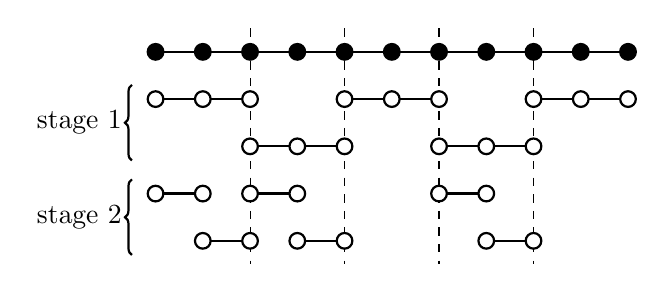
\begin{tikzpicture}[scale=.6]

        \foreach \i in {1, ..., 4}
        {
            \draw [dashed] (2 * \i, 0.5) -- (2 * \i, -4.5);
        }

        \draw [edge] (0,0) node [path vertex] {}
        \foreach \i in {1, ..., 10}
            {-- (\i, 0) node [path vertex] {} } ;

        \foreach \i in {0, ..., 4}
        {
            \draw let \n1 = {-1 - mod(\i, 2)} in
                    [edge] (2 * \i, \n1) node [query vertex] {}
                    --     ++(1, 0)      node [query vertex] {}
                    --     ++(1, 0)      node [query vertex] {};
        }

        \foreach \i in {0, 1, 3}
        {
            \draw [edge] (2 * \i, -3)   node [query vertex] {}
                  --     ++(1,  0)      node [query vertex] {}
                         ++(0, -1)      node [query vertex] {}
                  --     ++(1,  0)      node [query vertex] {};
        }

        \draw [decorate, decoration={brace}, thick]
              (-0.5, -2.3) -- (-0.5, -0.7)
              node [left, midway]{stage 1};
        \draw [decorate, decoration={brace}, thick]
              (-0.5, -4.3) -- (-0.5, -2.7)
              node [left, midway]{stage 2};
    \end{tikzpicture}
    \caption{Input instance corresponding to the string $11010$.}
    \label{fig:lower-bound-instance}
\end{figure}


\chapter{Offline Algorithms with Advice}
\label{chapter:offline}
The model of algorithms with advice appears to be a useful tool to give a
quantitative measure on the difficulty of online problems, which is more
fine grained than what competitive analysis alone offers. A new question
arises: Is it possible to use advice complexity to quantify the difficulty
of hard offline problems?

The concept of a Turing machine with advice is nothing new -- it has been
introduced in \cite{karp-advice}. However, the motivation behind the
Karp-Lipton model of advice differs significantly from ours -- their model
is closely tied to Boolean circuits and it requires that given a Turing
machine $A$, for every number $n \in \N$ there be some advice string
$\alpha_n$ such that for every input $x$ of size $n$, $A(x, \alpha_n)$
gives the correct answer.

Our interest lies somewhere else: We want to find out what amount of
additional information about a specific input instance can help an
algorithm -- or a Turing machine -- to perform better in terms of time or
space complexity. In other words, while Karp and Lipton allow only a
single advice string for a given size of input, we allow an advice string
specially tailored to each input instance.

The purpose of this chapter is not to give any conclusive results.
Instead, our intention is to lay out the groundwork for future research in
this area.

\section{Formal Definition of the Model}
\label{section:offline-definition}
There is a wide collection of computational models from which we can
choose one to extend with advice. We pick Turing machines due to their
status of the de-facto standard computational model.

\begin{definition}[Turing Machine with Advice]\label{definition:turing-advice}
    A \emph{Turing machine with advice} is a deterministic Turing machine
    $A$ with alphabet $\Sigma = \{0,1\}$, two read-only tapes and one
    read-write tape such that one read-only tape contains the input word
    and the other one contains an infinite binary advice string. $A$
    accepts an input word $x$ if there exists an advice string $\phi$ such
    that when the input tape contains $x$ and the advice tape contains
    $\phi$, $A$ terminates in an accepting state.

    A \emph{Turing machine with advice and output} has an additional
    write-only output tape. Let $S$ be some subset of $\Sigma^*$ and let
    $f: S \to \Sigma^*$ be some function. Turing machine $A$ computes the
    function $f$ if for each $x \in S$, there is an advice string $\phi$
    such that if the input tape contains $x$ and the advice tape contains
    $\phi$, $A$ writes $f(x)$ to the output tape and terminates in an
    accepting state.
\end{definition}

The same considerations as in the case of online algorithms apply here as
well. We define the model to use an infinite advice tape in order to avoid
giving away any additional information in the form of the length of
advice.

This definition resembles nondeterministic Turing machines and, in a
sense, it is equivalent -- it is easy to see that one computational step
of a nondeterministic Turing machine $A$ with $k$ possible outcomes can be
simulated by $\ceil{\log{}k}$ computational steps of a Turing machine $B$
with advice. In each step, $B$ reads one bit of advice and after reading
all $\ceil{\log{}k}$ bits, decodes the number $k$ indicating which
decision to take. Conversely, we can easily simulate a Turing machine $B$ with
advice using a nondeterministic Turing machine $A$: $A$ can simply
nondeterministically fill one tape used to emulate the advice tape with a
string of nondeterministically chosen length and then proceed to simulate
$B$ without any further changes. The key difference is, as we will see in
a little while, that the model with advice gives us fine-grained control
over how much information the machine can obtain nondeterministically.

The definition of a Turing machine with output is somewhat peculiar. Since
the result of a computation of a given machine $A$ with a given input $x$
can vary depending on the advice string, it is practically impossible to
determine what function $A$ computes. Instead, we choose the opposite
direction. In our work we concentrate on problems for which we know what
the expected output looks like, i.e., we already have a function $f$ and
we want to find a machine such that it can reach the correct output if it
receives correct advice.

It is easy to modify the definition of a machine with output to make it
better suited for analysis of optimization algorithms. Instead of
requiring that the machine computes the correct output, we can define a
cost function whose value is $\infty$ for invalid outputs (or $-\infty$,
depending on whether we talk about a minimization or maximization problem)
and define the output as the outcome with the minimal (or maximal) cost.

Let us now define the complexity measure which led to the conception of
this computational model in the first place.

\begin{definition}[Offline Advice Complexity]\label{definition:offline-advice-complexity}
    The \emph{advice complexity} of Turing machine $A$ with advice is a
    function $b: \N \to \N$ such that for every input $x$ such that $|x| =
    n$, $A$ accesses at most $b(n)$ positions on the advice tape.
\end{definition}

This complexity measure is analogous to the measure of space complexity in
nondeterministic Turing machines \cite{nspace}, except we are only
interested in the advice tape; on the work tape, $A$ can use as much space
as it needs to. Also note that while the space complexity of a Turing
machine is usually defined in a way that allows any multiplicative
constant, this is not the case of advice complexity. The reason is that
in the case of traditional space complexity, the linear tape compression
theorem holds \cite{tape-compression}, and even though it is possible to
represent multiple advice symbols in one position by extending the advice
alphabet in a similar way, we are specifically interested in the amount of
advice information in terms of the number of bits.


\chapter*{Conclusion}
\addcontentsline{toc}{chapter}{Conclusion}
\label{chapter:conclusion}
\input{tex/96conclusion.tex}

%\backmatter fixme: preco to tu nefunguje? asi chyba nejaky package

\todo{Make the bibliography consistent.}
\printbibliography

\appendix

%\chapter{Implementation}
%\input{tex/50implementation.tex}

\end{document}
